
%\documentclass{book}
\documentclass[a4paper,12pt]{scrartcl}


\usepackage[utf8x]{inputenc}
\usepackage[francais]{babel}
\usepackage{amsfonts}
\usepackage{tikz}
\usepackage{float}
\usepackage{graphicx} 
\usepackage{wrapfig}
\usepackage{url}
\usepackage{listings}

\usetikzlibrary{arrows,decorations.pathmorphing,backgrounds,fit,positioning,shapes.symbols,chains}


\title{Mercury Project}
%\author{Mathieu Simeral\\Antoine De Maleprade\\Rimbaut Saulignac\\Quentin Cormier\\\\Animateur : Thibault Raboisson}
%\date{\today}


\begin{document}  
    \thispagestyle{empty}
    \begin{figure}[H]
\includegraphics[height=85px, width=300px]{Photos_Mercury/eurekapluslogo.jpg}\end{figure}


    \begin{center}
      \Huge{\bf{Mercury Project}} \\
      \small{
      Mathieu Simeral\\Antoine De Maleprade\\Rimbaut Saulignac\\Quentin Cormier\\

      Animateur : Thibault Raboisson
      }
    \end{center}

    \begin{figure}[H]
		\begin{center}
		    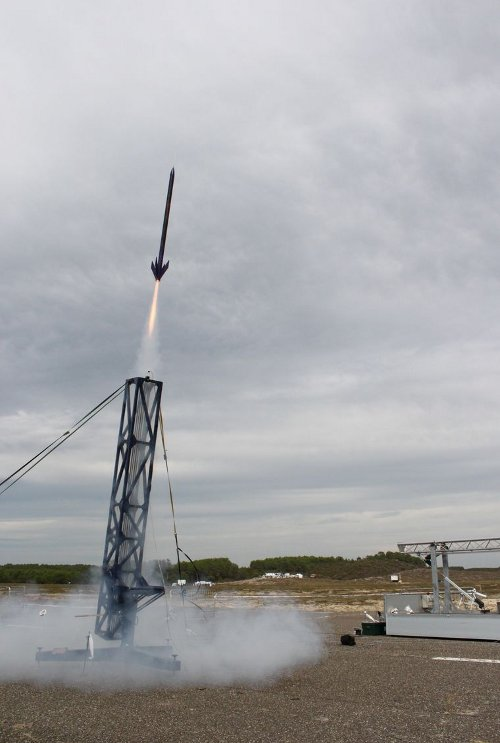
\includegraphics[height=250px, width=168px]{Photos_Mercury/decollage.jpg}
		\end{center}
    \end{figure}


    \begin{figure}[H]
      \begin{center}
	
\includegraphics[height=81px, width=400px]{Photos_Mercury/eurekaplus_partenaires_2010.jpg}
      \end{center}
    \end{figure}	

	
    \newpage
    \tableofcontents
    \newpage
	  \section{Introduction}
	      \subsection{But de la fusée}
		Mercury est une fusée expérimentale initiée en septembre dont le but est de mesurer le coefficient de pénétration dans l'air, 
		le $C_x$ de la fusée.

		En effet, la résistance de l'air d'une fusée peut être estimée par la formule : 
		$$ R_{air} = 0.5 * C_x * \rho_{air} * S * v^2$$

		Dans les logiciels de simulation de vol tel que Traject, Trajecto, etc, on donne arbitrairement pour $C_x$ une valeur comme 0,7 ou 0,8.
		Cette expérience pourrait donc permettre d'avoir une vraie valeur expérimentale du $C_x$, dans les conditions de vol de la fusée.

	      \subsection{Équipe du projet}
		 \begin{itemize}
		  \item \textsc{Mathieu Simeral (14 ans)} : Responsable de la mécanique, réalisation de tous les plans de la fusée, ainsi que du parachute.
		  \item \textsc{Rimbaut Saulignac (15 ans)} : Responsable de la mécanique avec Mathieu.
		  \item \textsc{Antoine Demaleprade (17 ans)} : Responsable de l'électronique de l'expérience et de la stabilité de la fusée\footnote{Et bien plus encore}.
		  \item \textsc{Quentin Cormier (17 ans)} (Chef de projet) : J'ai réalisé la minuterie, les calculs du ressort\footnote{Et je suis donc responsable du ``système cassé en 0.1 sec''}, le système de l'expérience, ainsi que ce dossier.
		  \item \textsc{Thibault Raboisson} : Président de l'association Eurêka+, Thibault nous a encadrés et a toujours su trouver des solutions pertinentes et rapides à nos problèmes \footnote{Oui, l'idée de mettre les ailerons à l'envers, c'est lui}
		 \end{itemize}

		\begin{figure}[H]
		    \caption{Les membres d'Eureka+ au complet}
		    \begin{center}
		      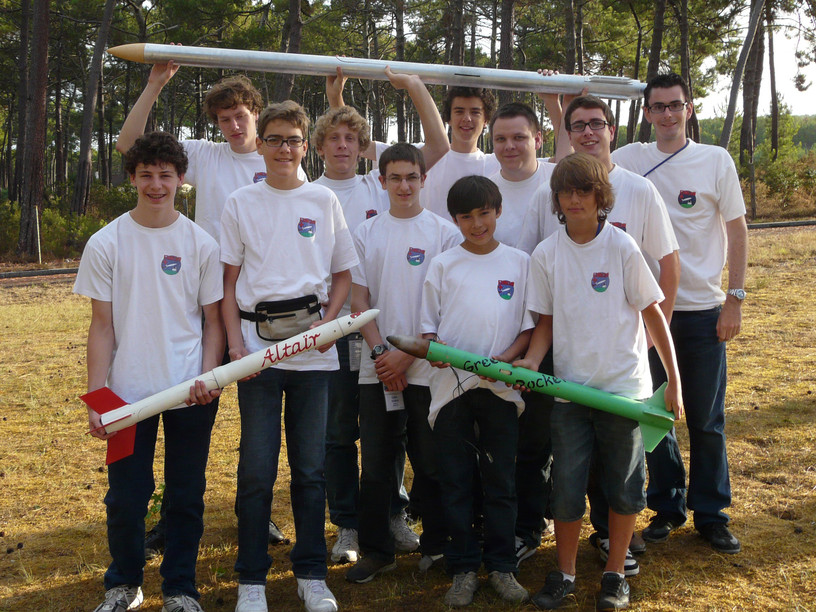
\includegraphics[height=188px, width=250px]{Photos_Mercury/cspace2010_equipe_EUREKA_PLUS.jpg}
		    \end{center}
		\end{figure}
	 \newpage	
	   \section{Expérience}
	   
	   	Note : les calculs du Cx et le dimensionnement du ressort sont faux : ils ont été réalisés avec des connaissances de Terminale. J'ai jugé bon de laisser ces calculs qui permettent de comprendre l'échec de l'expérience.
	   	Des calculs plus justes pourront être trouvés dans l'annexe en fin de document.
	  
             \subsection{Valeurs mesurées }

		Pour mesurer expérimentalement le $C_x$ de la fusée, nous allons mettre un ressort sur lequel va pousser le propulseur.
		\begin{figure}[H]
		  \begin{center}
		    \caption{Schéma du ressort dans la fusée}
		    \begin{tikzpicture}[scale=.3]
			\draw (-1,0) to [out=90, in=90] (0,5)
						 to [out=90, in=90] (1,0);
			\draw (-1,0) rectangle (1,-20);
			\foreach \x in {-9, -9.5, -10, -10.5, -11, -11.5} \draw (0,\x) circle (0.8);
			\draw[fill=white] (-0.7,-12) rectangle (0.7,-21);

			\draw[line width=1pt] [->] (1.5,-18) -- (1.5,-12);
			\draw (10,-14) node[below left] {Propulseur};

			\draw[line width=1pt] [->] (1.5,-5) -- (1.5,-9);
			\draw (9,-6) node[below left] {$R_{air} + P_f$};

		    \end{tikzpicture}
		  \end{center}
		\end{figure}
		\floatplacement{figure}{t}


		Les deux forces qui s'appliquent de part et d'autre du ressort sont d'un coté la poussée du propulseur, et de l'autre la somme résistance de l'air ($R_{air}$) + poids de la fusée dans l'axe de la fusée ($P_f$).
		La poussée du propulseur étant la force la plus grande, le ressort mesure donc $V = R_{air} + P_f$.
		
		Si on note $\alpha$ l'angle de la fusée par rapport au sol, alors on a : 
		  $$ P_f = m * g * \cos{(90-\alpha)}$$
		D'où : 
		  $$ P_f =  m * g * \sin{\alpha}$$		
		On a donc 
		  $$ R_{air} = V - ( m * g * \sin{\alpha})$$
		  $$ \Leftrightarrow 0.5 * C_x * \rho_{air} * S * v^2 = V - m * g * \sin{\alpha} $$
		D'où
		  $$ C_x = \frac{2(V - m * g * \sin{\alpha})}{\rho_{air} * S * v^2} $$
		
		On mesure l'angle de la fusée avec un capteur d'accélération 3 axes, la vitesse de la fusée avec ce même capteur couplé à un capteur de pression (en utilisant la méthode d'Euler).
		V est obtenu en mesurant l'élongation du ressort sur le propulseur à l'aide d'un potentiomètre linéaire.
		\begin{figure}[H]
		    \begin{center}
			\caption{ Maquette de l'expérience pour la présentation du projet en début d'année}
			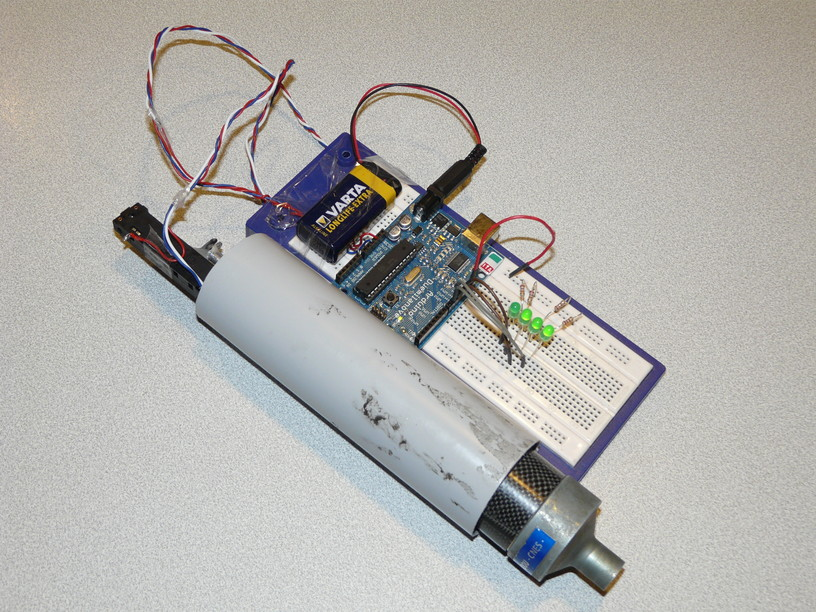
\includegraphics[height=244px, width=326px]{Photos_Mercury/maquette_systeme_ressort.jpg}
		     \end{center}
		\end{figure}
		\begin{figure}[H]
		    \begin{center}
			\caption{ Système de l'expérience finalisée en fin d'année }
			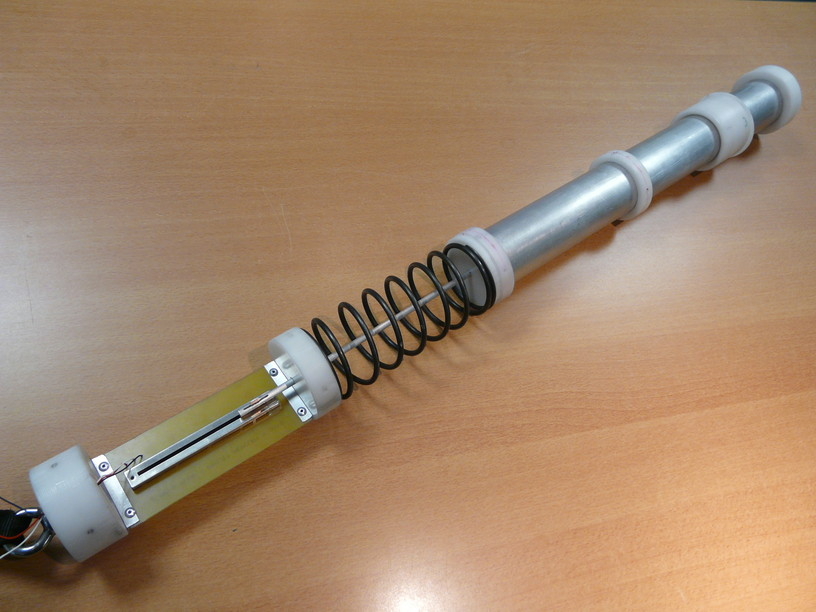
\includegraphics[height=244px, width=326px]{Photos_Mercury/systemeressort.jpg}
		     \end{center}
		\end{figure}

	\subsection{Calcul du ressort}
	    \subsubsection{Forces que subit le ressort}
	      Le but est de déterminer quel ressort commander pour mesurer le plus précisément possible la somme de la 
	      résistance de l’air et du poids selon l’axe de la fusée.
	      \\
	      \begin{figure}[H]
		  \begin{center}
		    \caption{Forces qui s'appliquent de chaque coté d'un ressort}
		    \begin{tikzpicture}[scale=.3]
			\foreach \x in {-1, -0.5, 0, 0.5, 1} \draw (\x,0) circle (0.8);
			\draw[line width=1pt] [->] (-4,0) -- (-2,0);
			\draw (-2.5,0) node[below left] {$\vec{f_1}$};

			\draw[line width=1pt] [->] (4,0) -- (2,0);
			\draw (4,0) node[below left] {$\vec{f_2}$};
		    \end{tikzpicture}
		  \end{center}
		\end{figure}
		\floatplacement{figure}{t}
	      Lorsque deux forces $\vec{f_1}$ et $\vec{f_2}$ de normes respectives $F_1$ et $F_2$ s'appliquent de chaque coté d’un ressort, 
	      la norme de la force que subit le ressort est égale à :   
		$$ \min(F_1, F_2)$$


	      Dans notre cas, la force la plus faible est la résistance de l’air + le poids dans l’axe de la fusée, $R_{air} + P_f$.
	    \subsubsection{Calcul de la force maximale subie}
	      Une feuille de calcul trajecto nous montre que $R_{air} + P_f$ est toujours plus faible que la poussée du propulseur.
	      On cherche donc le maximum de  : $$R_{air} + P * \sin{\alpha}$$
    
	      Cela correspond au maximum de la résistance de l’air, soit le maximum de la vitesse de la fusée.
	      Avec une masse de 9,5kg, une surface de coupe de $6227 mm^2$, et un $C_x$ de 0.7, 
	      on trouve une vitesse maximum de $180 m.s^{-1}$ correspondant à un angle de 76.36\degre : 
	      \begin{figure}[H]
		    \begin{center}
		      \caption{ Vitesse max et angle correspondant, données trajecto }
		      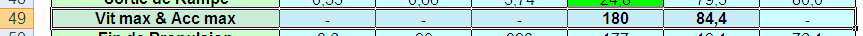
\includegraphics[height=15px, width=400px]{Photos_Mercury/vmax.png}
		      \vskip1em
		      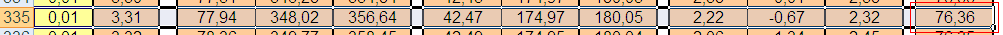
\includegraphics[height=15px, width=400px]{Photos_Mercury/angle.png}
		    \end{center}
	      \end{figure}

	      On trouve donc une résistance de l’air maximale de :
	      $$R_{air} = 0.5*0.7*0.006227*1.225*180² = 86.5 N$$
	      Et un poids selon l’axe de la fusée de : 
	      $$P_f = 9.5*9.81*\sin{76.36} = 90.6 N$$
	      Donc la force que doit supporter le ressort est de $90.6+86.5 = 177.1 N$.

	      A ceci s'ajoute les 20\% de marge de sécurité : 
	      $$V = 177,1 * 1,2 = 212,5 N$$

	      Finalement, nous avons choisi un ressort de 230N.
	      \subsubsection{Constante k du ressort}
	      Le propulseur pousse sur le ressort, qui pousse sur un potentiomètre.\\
	      On mesure la tension du potentiomètre linéaire qui correspond à la compression du ressort.
	      Notre potentiomètre fait 8cm, donc, quand on pousse 230 N sur notre ressort, il doit s’être compressé de 8cm.
	      Nous avons donc une constante k du ressort de : 
	      $$k = 230/(8*10-2) = 2875 N.m^{-1}$$
		\begin{figure}[H]
		    \begin{center}
		      \caption{Schéma du ressort commandé (données constructeur) }
		      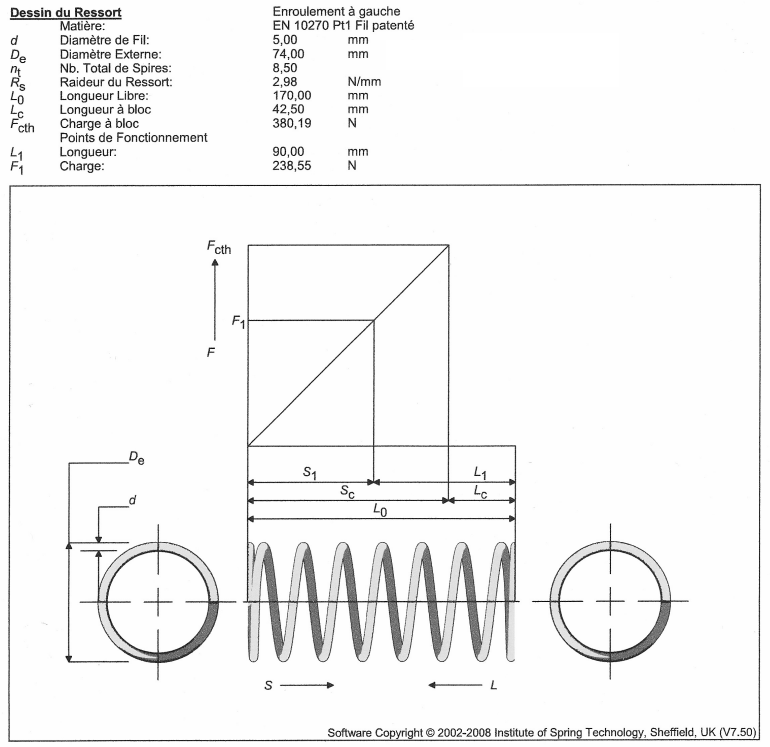
\includegraphics[height=400px, width=400px]{Photos_Mercury/ressort.png}
		    \end{center}
		\end{figure}
 

	\subsection{Électronique de l'expérience}
		L'électronique de l'expérience est basée sur une arduino.\\

		Nous avions prévu de mettre un capteur d'accélération numérique 3 axes, ainsi qu'un capteur de pression analogique\footnote{``MPX5100AP``, chez Farnell}, en plus du ressort.
		Durant la campagne, nous avons décidé d'émettre les données avec un émetteur Kiwi, fournit par le \textsc{cnes}. \\

		Cependant alors que la fusée était entièrement prête, à une nuit du lancement, le capteur d'accélération a cessé de fonctionner.
		Dans la précipitation, nous avons trouvé un club qui nous a donné un gyroscope analogique 2 axes\footnote{``Dual axis IXZ-500'', voir ici : http://www.sparkfun.com/products/9410.} qui a été monté et intégré dans la nuit.
		
		Ainsi, dans la version qui a volé de la fusée, nous avons un gyroscope deux axes, un capteur de pression et le potentiomètre du ressort.
		
		Le tout est enregistré dans la fusée sur une carte SD, et envoyé en télémesure avec l'émetteur kiwi.
	      \subsection{Mécanique de l'expérience}	
	      Le corps de la fusée est un tube de diamètre 80 mm en aluminium.
	      Le propulseur (fixé dans un tube de 60 min de diamètre) coulisse dans le corps de la fusée grâce à des bagues en plastique.
	      
	      Les bagues ont été réalisées avec le nouveau tour à métaux de l'association.
	     \begin{figure}[H]
		    \begin{center}
		      \caption{Mercury inaugure le tour de Eurêka+}
		      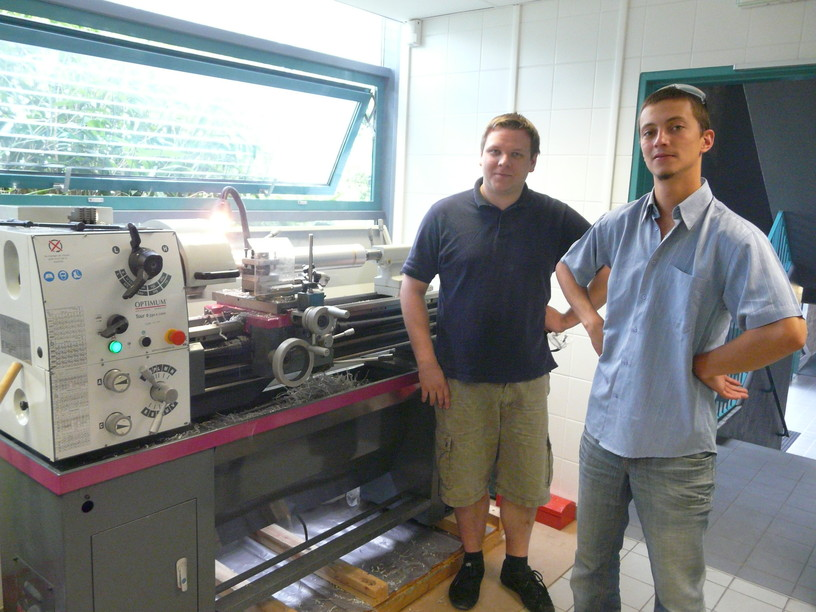
\includegraphics[height=244px, width=326px]{Photos_Mercury/tour.jpg}
		    \end{center}
	      \end{figure}

	     \begin{figure}[H]
		    \begin{center}
		      \caption{Les bagues qui guident le tube du propulseur dans le tube de la fusée}
		      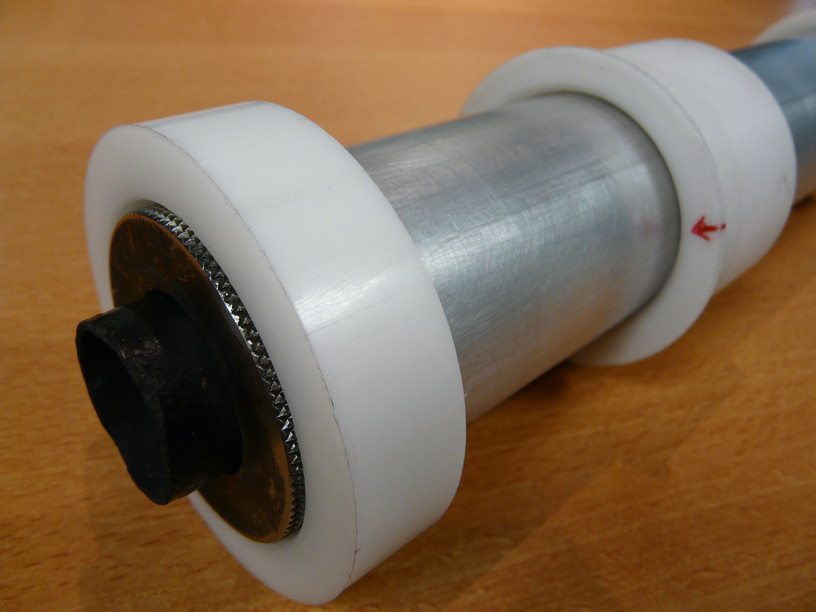
\includegraphics[height=244px, width=326px]{Photos_Mercury/bague_propulseur.jpg}
		    \end{center}
	      \end{figure}



		\begin{figure}[H]
		  \begin{center}
		    \caption{Électronique de l'expérience}
		\centering
		  \begin{tikzpicture}
		    [node distance = 1cm, auto,font=\footnotesize,
		    % STYLES
		    every node/.style={node distance=3cm},
		    % The comment style is used to describe the characteristics of each force
		    comment/.style={rectangle, inner sep= 5pt, text width=4cm, node distance=0.25cm, font=\scriptsize\sffamily},
		    % The force style is used to draw the forces' name
		    force/.style={rectangle, draw, fill=black!10, inner sep=5pt, text width=4cm, text badly centered, minimum height=1.2cm, font=\bfseries\footnotesize\sffamily}] 

		    % Draw forces
		    \node [force] (arduino) {Arduino};
		    \node [force, above of=arduino] (gyro) {Gyroscope deux axes};
		    \node [force, left=1cm of arduino] (pression) {Capteur de pression};
		    \node [force, right=1cm of arduino] (ressort) {Compression du ressort};
		    \node [force, below of=arduino] (modulateur) {Modulateur FSK};
		    \node [force, below of=modulateur] (telem) {Emetteur FSK ``Kiwi''};
 		    \node [force, below of=arduino, right=1cm of arduino] (cartesd) {Carte SD};
	
		    \node [force, text width=3cm, dashed, left=1cm of gyro] (alim) {Alimentations};
		    \node [force, text width=3cm, dashed, below= 0.2cm of alim] (int) {Interrupteurs};
		    % Draw the links between forces
		    \path[->,thick] 
		    (gyro) edge (arduino)
		    (pression) edge (arduino)
		    (ressort) edge (arduino)
		    (arduino) edge (modulateur)
		    (modulateur) edge (telem)
		    (arduino) edge (cartesd);
		    \end{tikzpicture} 
		  \end{center}
		  \end{figure}
		  \floatplacement{figure}{t}
	 \newpage

	\section{Réalisation de la fusée}
		\subsection{Plan général de la fusée}

		\begin{figure}[H]
		  \begin{center}
		    \caption{Schéma des élements de  la fusée}
		    \begin{tikzpicture}[scale=.3]
			\draw (-1.5,0) to [out=90, in=90] (0,5)
						 to [out=90, in=90] (1.5,0);
			\draw (-1.5,0) rectangle (1.5,-17);
			\draw (-1.5,-17) rectangle (1.5,-30);
			\draw (-1.5,-30) rectangle (1.5,-50);

			\foreach \x in {-33.5, -34, -34.5, -35, -35.5, -36} \draw (0,\x) circle (1.3);
			
			\draw[fill=white] (-1,-1) rectangle (1,-5);
			\draw[fill=white] (-1,-5) rectangle (1,-12);
			\draw[fill=white] (-1,-12) rectangle (1,-16);

			\draw[fill=white] (-1,-30.5) rectangle (1,-33.5);
			\draw[fill=white] (-1,-37) rectangle (1,-53);


			\draw[line width=1pt] [<->] (2,-37) -- (2,-53);
			\draw (5,-43.5) node[right] {Propulseur dans son tube};

			\draw[line width=1pt] [<->] (2,-33.5) -- (2,-37);
			\draw (5,-34.5) node[right] {Ressort};		

			\draw[line width=1pt] [<->] (2,-30.5) -- (2,-33.5);
			\draw (5,-31.5) node[right] {Potentiomètre};		

			\draw[line width=1pt] [<->] (2,-17) -- (2,-30);
			\draw (5,-24) node[right] {Case parachute, porte};	

			\draw[line width=1pt] [<->] (2,-1) -- (2,-5);
			\draw (5,-2.5) node[right] {Électronique émetteur};	


			\draw[line width=1pt] [<->] (2,-5) -- (2,-12);
			\draw (5,-8.5) node[right] {Électronique expérience};

			\draw[line width=1pt] [<->] (2,-12) -- (2,-16);
			\draw (5,-14) node[right] {Minuterie};	

			\draw[line width=1pt] [<->] (2,5) -- (2,0);
			\draw (5,2.5) node[right] {Ogive : antenne émetteur};	



	




		    \end{tikzpicture}
		  \end{center}
		\end{figure}
		\floatplacement{figure}{t}


		\subsection{Estimation de la masse de la fusée}
	      On estime la masse de la fusée en pesant chaque élément séparément. \\\\
	    \begin{tabular}{{|c|c|}}
	       \hline
	      Objet & Masse \\
	      \hline
	      Tube de la fusée & 2760 g \\
	      Tube de l'expérience & 502.5 g \\	 
	      Ogive & 66 g \\	
	      Structure : structures, cartes, plaque piles & 670 g \\	 
	      Aimant & 130 g \\	 
	      8 piles & 400 g \\	 
	      Arduino & 50 g \\	   
	      Séparateurs & 80 g \\	   
	      Anneaux & 970 g \\	   
	      Propulseur vide & 650 g \\	   
	      Ressort & 320 g \\	   
	      Ailerons (x4) & 1600 g \\	   
	      \hline
	      Total & 8 kg (à vide) $\pm{1 kg}$ \\	
	       \hline
	    \end{tabular} \\\\
	    Une fois terminée, la fusée faisait 7,2 kg.

	           \subsection{Le parachute}
	      La masse estimée de la fusée est de 8 kg, $ g = 9.81 m.s^{-2}$, $ \rho_{air} = 1.2 kg.m^{-3} $, $ C_x = 1  $, 
	      $ V_{impact} = 10 m.s^{-1} $. \\\\
	      \subsubsection{Calcul de la surface}
		La vitesse de la fusée $V_{impacte}$ à l'impact est reliée à la surface du parachute $S$ par la relation : 
		$$ V_{impact} = \sqrt{\frac{2*m*g}{\rho_{air}*C_x*S}} $$
	      D'où : 
		$$ S = \frac{2*m*g}{\rho_{air}*C_x*(V_{impact})^2} $$
	      Application Numérique : 
		$$ S = \frac{2*8*9.81}{1.225*10^2} \approx 1.5 m^2$$
	      
	      \subsubsection{Réalisation du parachute}

	      Nous utilisons un parachute en croix constitué de 5 carrés de même aire. La surface d'un carré est donc donnée par : 
		$$S_{carre} = \frac{1.5}{5} = 0.3m^2 $$
		D'ou la longueur d'un coté est donné par : 
		$$l_c = \sqrt{0.3} \approx 0.5m $$
		\begin{figure}[H]
		  \begin{center}
		    \caption{Schéma du parachute}
		      \begin{tikzpicture}[scale=2]
			\draw[fill=white] (0,0) rectangle (1,1);
			\draw[fill=white] (0,1) rectangle (1,2);
			\draw[fill=white] (0,-1) rectangle (1,0);
			\draw[fill=white] (-1,0) rectangle (0,1);
			\draw[fill=white] (1,0) rectangle (2,1);
			\draw[|<->|] (0,-1.2) -- (1,-1.2);
			\draw (0.9,-1.3) node[below left] {$l_c = 50 cm$};
		    \end{tikzpicture}
		  \end{center}
		\end{figure}
		\floatplacement{figure}{t}
	   \subsection{La minuterie}
		L'ouverture se fait avec un électroaimant inversé : quand on alimente l'électroaimant (en 24V), celui-ci cesse son champ magnétique.\\
		La minuterie compte le temps avec un 4060 (alimenté en 5V). Au bout du décompte, elle active un relais et alimente l'électroaimant.\\
		La porte s'ouvre, et le parachute se déplie.
	      \begin{figure}[H]
		    \begin{center}
		      \caption{ Schéma électronique de la minuterie }
		      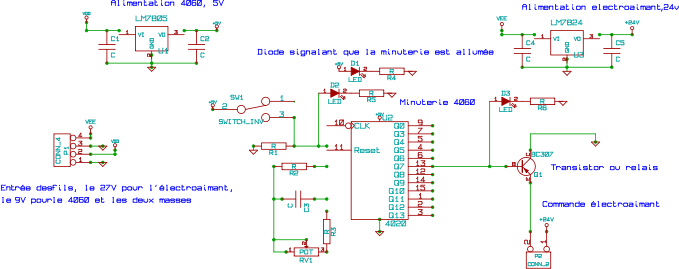
\includegraphics[height=147px, width=372px]{Photos_Mercury/4060.png}
		    \end{center}
	      \end{figure}
	      \begin{figure}[H]
		    \begin{center}
		      \caption{ Typon de la minuterie }
		      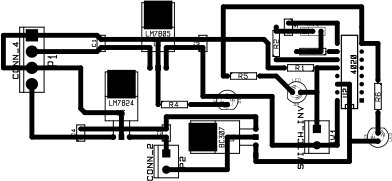
\includegraphics[height=181px, width=392px]{Photos_Mercury/4060-brd.png}
		    \end{center}
	      \end{figure}
		   Le circuit possède deux régulateurs de tension, qui produisent du 5V et du 24V, respectivement pour le 4060 et pour l'électroaimant.\\
		   Ils doivent être alimentés par du 9V et du 27V.
		   La minuterie requiert donc $3+1$ piles 9V.
		  
		   On règle le temps du décompte avec une résistance variable.\\
		   On a en effet : 
		    $$ f = \frac{1}{256 * 2.3 * R_t*C_t}$$
		   où : 
		    $$ C_t = 470 nF$$
		   On a donc 
		    $$ t = 256 * 2.3 * R_t * 470*10^{-9} $$
		   Ou encore : 
		    $$ R_t = \frac{t}{256 * 2.3 * 470 * 10^{-9}}$$
		   La commande de l'électroaimant se faisait à l'origine avec un transistor, mais nous l'avons remplacée par un relais.

	  \subsection{La trajectoire de la fusée}
	      La trajectoire de la fusée se calcule avec les formules de Newton\footnote{Voir ``Le vol de la fusée'', (document Planète-Sciences)}ou avec les logiciels de Planète-Science comme trajecto : 
	      \begin{figure}[H]
		    \begin{center}
		      \caption{ Trajectoire de la fusée, d'après le logiciel \textsc{Trajecto}}
		      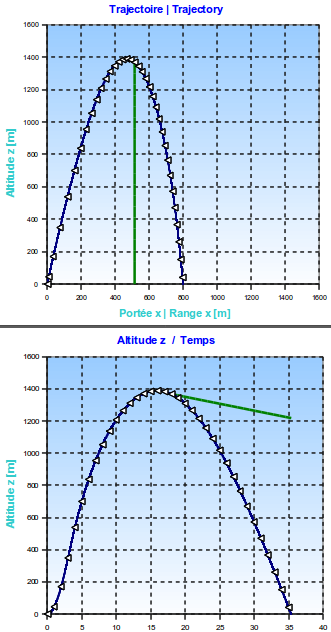
\includegraphics[height=316px, width=156px]{Photos_Mercury/courbe-trajectoire.png}
		    \end{center}
	      \end{figure}
	      D'après le logiciel, l'apogée serait atteinte à 1382m, au bout de 15.9 s, et la vitesse maximale serait de $202 m.s^{-1}$.
	  \subsection{La stabilité de la fusée}
	      
	    La stabilité de la fusée tient d'une anecdote assez amusante. Nous avions découpé/fixé les ailerons avant la campagne de Biscarrosse, en faisant une estimation grossière du centre de gravité.
	    Il s'est avéré que notre centre de gravité réel, une fois la fusée terminée se trouvait 7 cm en dessous de nos prévisions. Pour le baisser d'une telle distance, 
	    il aurait fallu rajouter une masse très importante tout en bas de la fusée, ce qui n'était pas envisageable avec toute l'expérience.\\
	    
	    Finalement, c'est Thibault qui a trouvé la solution : retourner les ailerons ! En effet, d'après stabilito, en mettant les ailerons a l'envers, la fusée redevient stable.
	      \begin{figure}[H]
		    \begin{center}
		      \caption{Les ailerons, à l'envers, c'est mieux (et ça fait peur au contrôle).}
		      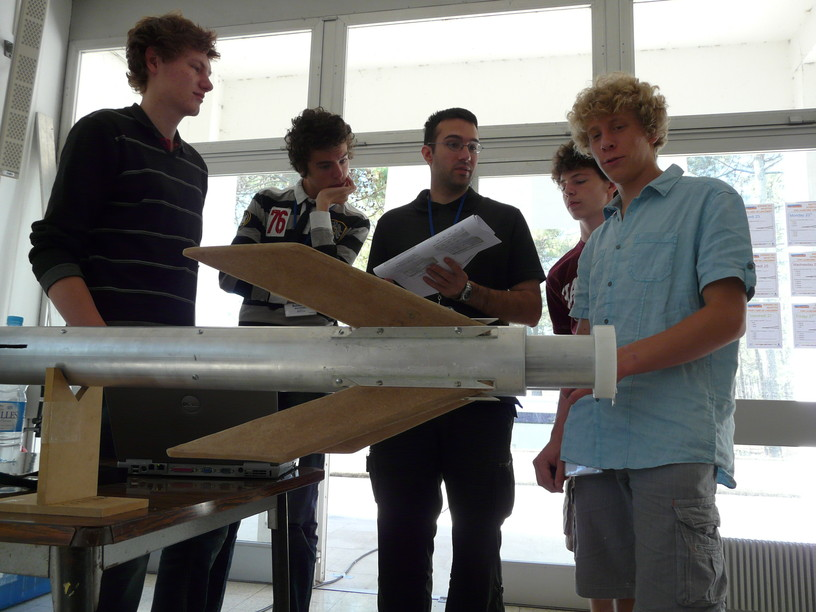
\includegraphics[height=244px, width=326px]{Photos_Mercury/ailerons-controles.jpg}
		    \end{center}
	      \end{figure}
	      
	     \begin{figure}[H]
		    \begin{center}
		      \caption{Résultat du calcul de la stabilité avec \textsc{Stabilito}}
		      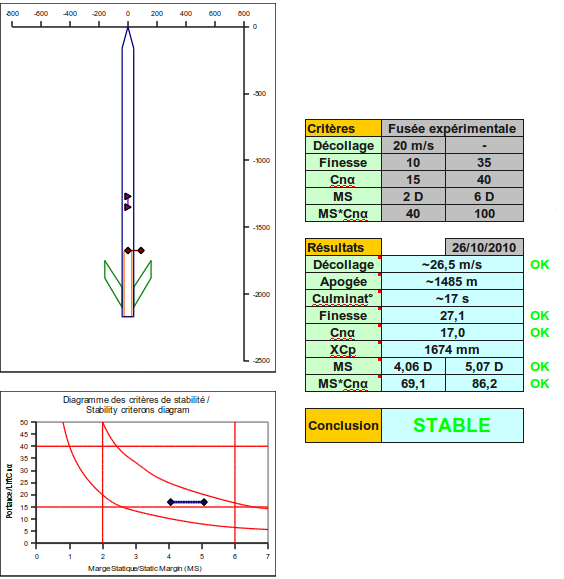
\includegraphics[height=289px, width=282px]{Photos_Mercury/stabilite.png}
		    \end{center}
	      \end{figure}

	  \subsection{Le montage de la fusée}
	   La fusée a été peinte dans la nuit qui a précédé le lancement.
	   Le lendemain, nous avons graissé le ressort, tout remonté, en suivant la chronologie, et nous sommes partis dans l'aire de lancement.

	 \newpage

	\section{La campagne de lancement}
	
	Nous avons participé à la campagne de lancement C'space dans les Landes au \textsc{CELM} à Biscarrosse.
	Cette semaine est la concrétisation du travail effectué tout au long de l'année.
	Une dizaine de membres de l'association Eurêka+ y ont participé pour y lancer 4 de leurs projets.
	Pour l'équipe Mercury l'objectif est de finaliser la fusée, de passer les qualifications pour procéder au vol de la fusée.

	  \subsection{Le vol}
	  
	  Le vol a eu lieu jeudi dans le début de l'après-midi, sur une rampe ``Obélix''. 	
	  Les ailerons à l'envers ont bien assuré la stabilité de la fusée.

	  Le parachute s'est correctement ouvert au bout des 15 secondes comme prévu.
	  Cependant, le parachute s'est mal déplié et la fusée a fait une torche, probablement à cause de la sangle trop courte qui retenait le parachute à la fusée.
	  
	  La fusée s'est enfoncée dans le sable au bout d'une minute de vol, ce qui a cassé la carte SD. Heureusement, la télémesure FSK a correctement fonctionné.
	  
	  Sur les vidéos du décollage qui ont été prises par différentes personnes de l'équipe de Planète-Sciences, on aperçoit que la butée de l'expérience saute alors même que la fusée n'est pas sortie de la rampe.
	  Nous avons donc sous-dimensionné le ressort, peut-être aurait-t-il fallu prendre en compte la grande énergie que libère l'impact entre le propulseur dans sa cage et le ressort au premier contact.
	  
	  La butée ayant sauté, le potentiomètre s'est cassé très rapidement et cette partie de l'expérience est donc un échec.
	  On pourra cependant analyser les données du gyroscope et du capteur de pression.


      	      \begin{figure}[H]
		    \begin{center}
		      \caption{Vol H-30min}
		      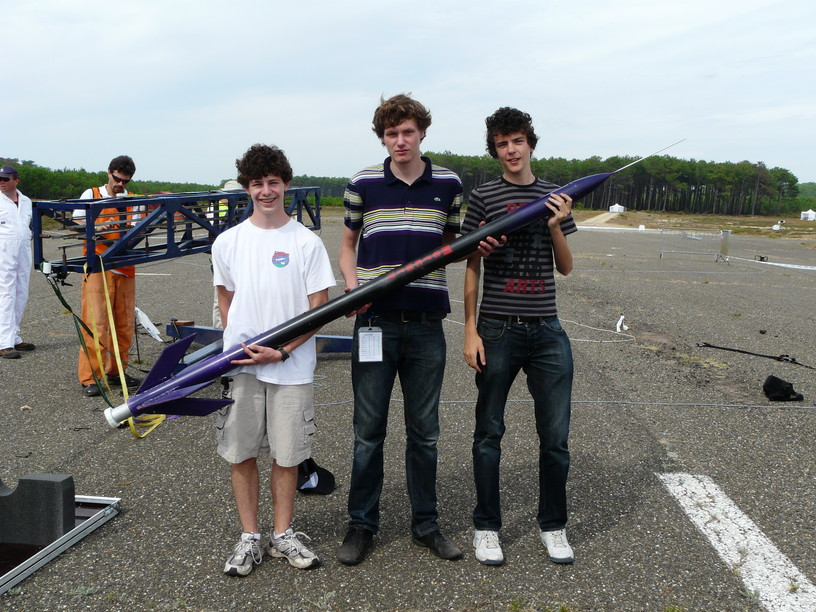
\includegraphics[height=244px, width=326px]{Photos_Mercury/pre_vol.jpg}
		    \end{center}
	      \end{figure}
      	      \begin{figure}[H]
		    \begin{center}
		      \caption{Mise en rampe de la fusée sur l'air de lancement}
		      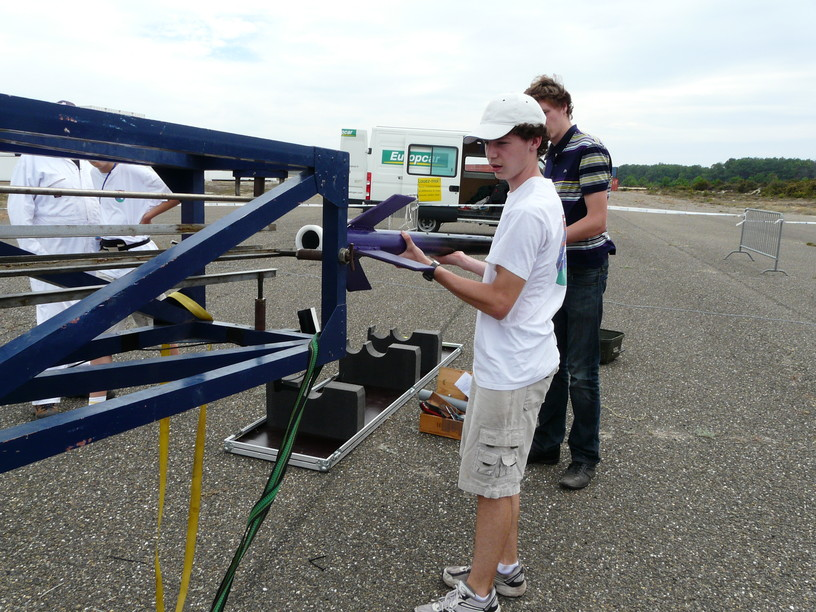
\includegraphics[height=244px, width=326px]{Photos_Mercury/miseenrampe.jpg}
		    \end{center}
	      \end{figure}
      	      \begin{figure}[H]
		    \begin{center}
		      \caption{Vol dans 1 min!}
		      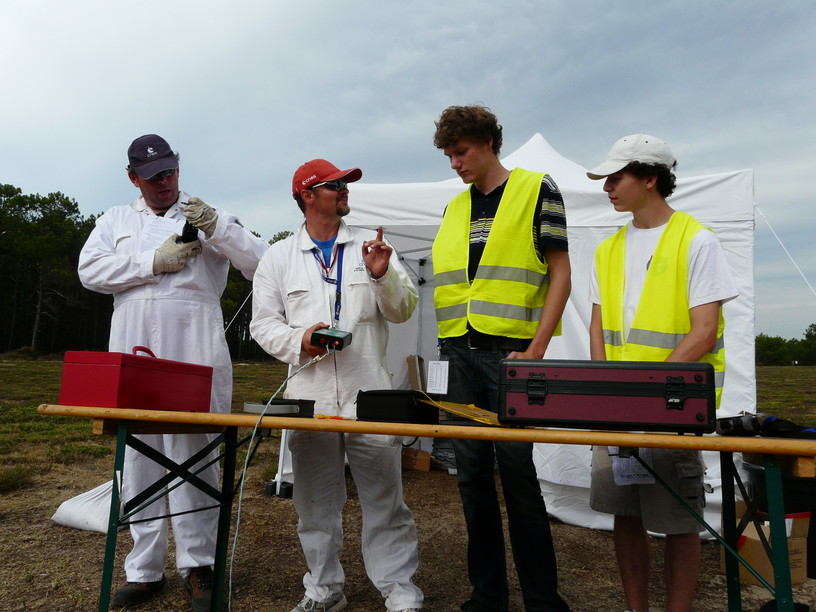
\includegraphics[height=244px, width=326px]{Photos_Mercury/volj-10s.jpg}
		    \end{center}
	      \end{figure}
      	      \begin{figure}[H]
		    \begin{center}
		      \caption{On retrouve la fusée, un peu abîmée.}
		      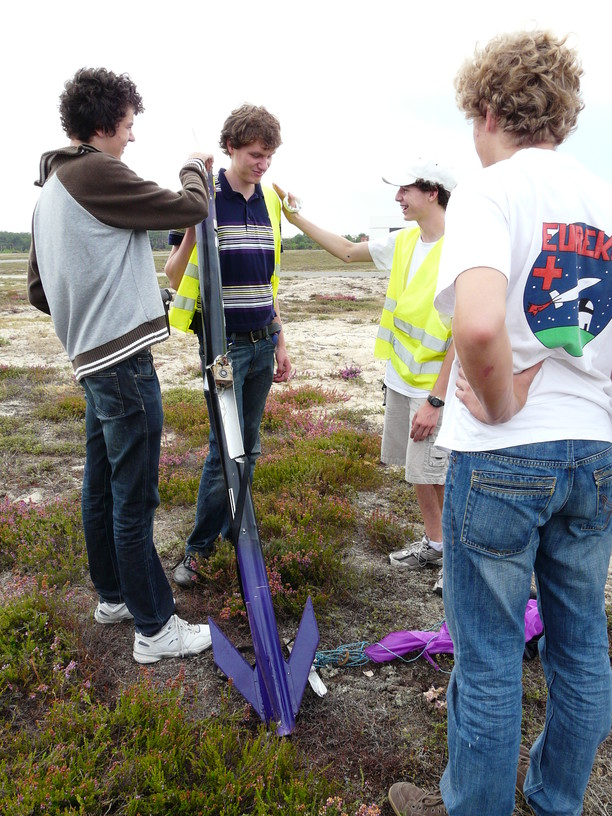
\includegraphics[height=326px, width=244px]{Photos_Mercury/resultat-vol.jpg}
		    \end{center}
	      \end{figure}
   	      \begin{figure}[H]
		    \begin{center}
		      \caption{Retour de l'équipe, un peu dépitée.}
		      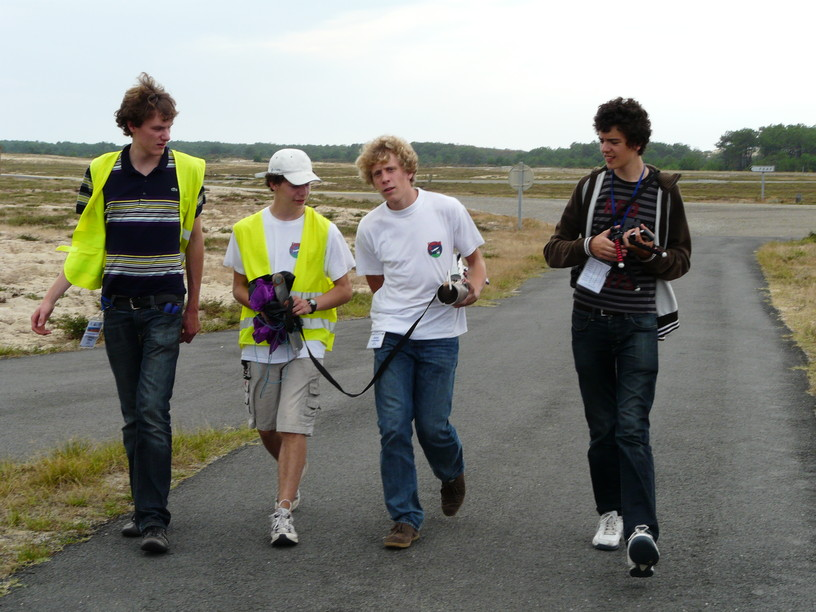
\includegraphics[height=244px, width=326px]{Photos_Mercury/retour.jpg}
		    \end{center}
	      \end{figure}

	  
	  \subsection{Analyse des données de l'expérience}
	
	  C'est Antoine qui s'est occupé de la récupération des données de la télémesure. Le vol a duré exactement 60 secondes.
	  \subsubsection{Capteur de pression}
	  On peut retrouver l'altitude avec le capteur de pression en utilisant la formule : $$ z = 44330.76924(\frac{p_0-p}{p_0})^{\frac{200}{1051}}$$ avec $p_0$ la pression initiale au niveau de la rampe, et p la pression. 
	  \begin{figure}[H]
		\begin{center}
		    \caption{ Courbe de la pression }
		    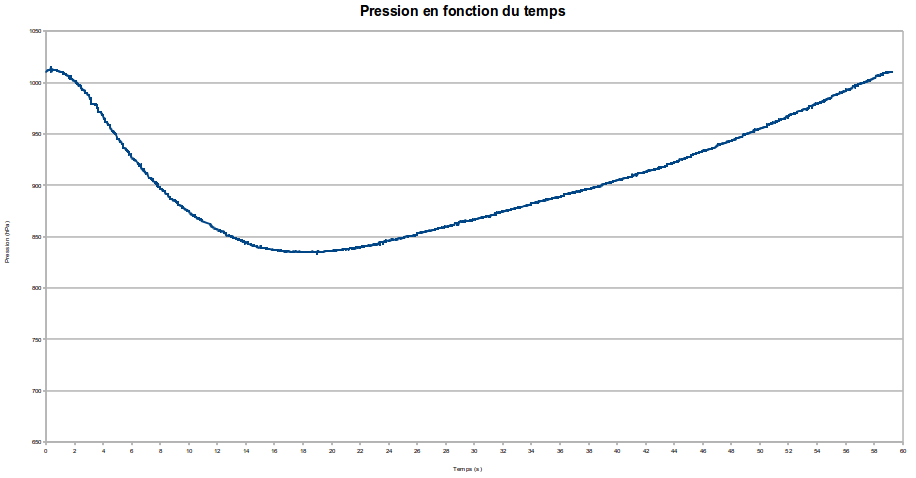
\includegraphics[height=236px, width=458px]{analyse/pression.png}
		\end{center}
	  \end{figure}
	  \begin{figure}[H]
		\begin{center}
		    \caption{ Courbe de l'altitude }
		    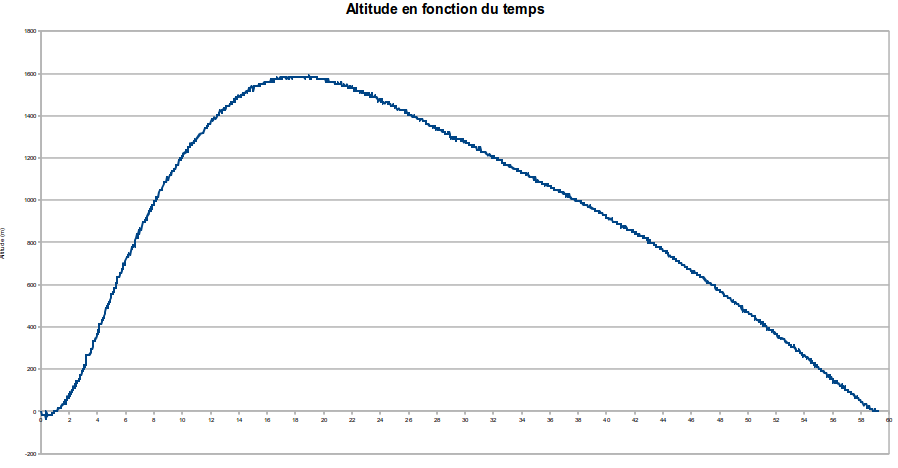
\includegraphics[height=234px, width=449px]{analyse/altitude.png}
		\end{center}
	  \end{figure}
	  L'apogée a été atteinte à 15.9 sec, et correspond à une hauteur de 1580m.
	  
	  \subsubsection{Gyroscope}
	  Le gyroscope nous permet d'avoir la vitesse angulaire dans l'axe x et dans l'axe y.
	  \begin{figure}[H]
		\begin{center}
		    \caption{ Vitesse angulaire en x et en y en fonction du temps }
		    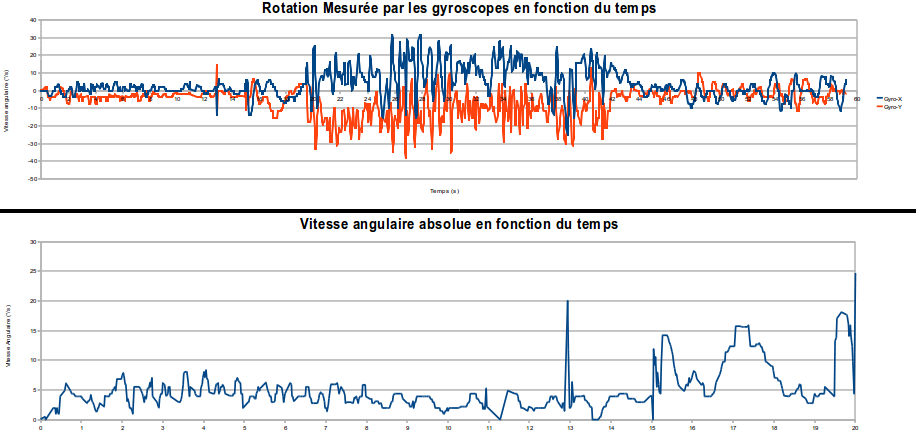
\includegraphics[height=219px, width=458px]{analyse/rotation-vitesse-angulaire.png}
		\end{center}
	  \end{figure}
	  On intégre la vitesse angulaire de l'axe y ($\theta_0 = 80°$) avec la méthode d'Euler pour avoir l'angle par rapport au sol en fonction du temps.
	  \begin{figure}[H]
		\begin{center}
		    \caption{ Angle par rapport au sol }
		    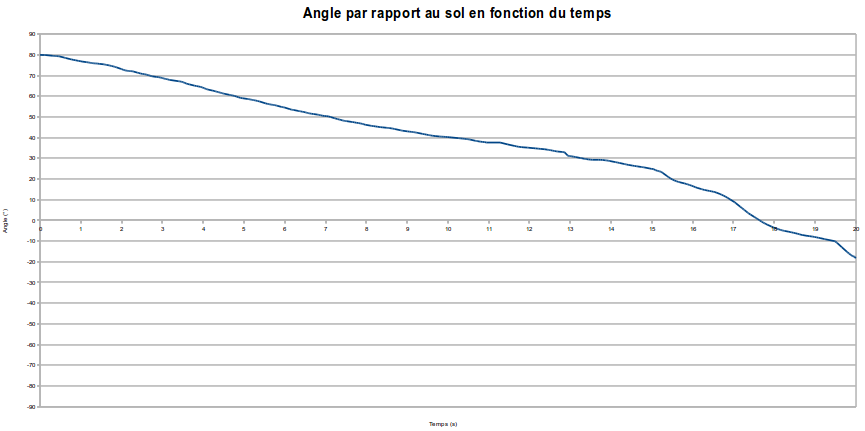
\includegraphics[height=215px, width=432px]{analyse/angle.png}
		\end{center}
	  \end{figure}	
	  A l'apogée, nous avions un angle de 25°.
	  \subsubsection{Potentiomètre}
	  La potentiomètre a cassé au bout de 0.1 sec, il n'y a donc pas de données valables pour cette expérience.
	  \begin{figure}[H]
		\begin{center}
		    \caption{ Compression du ressort en fonction du temps }
		    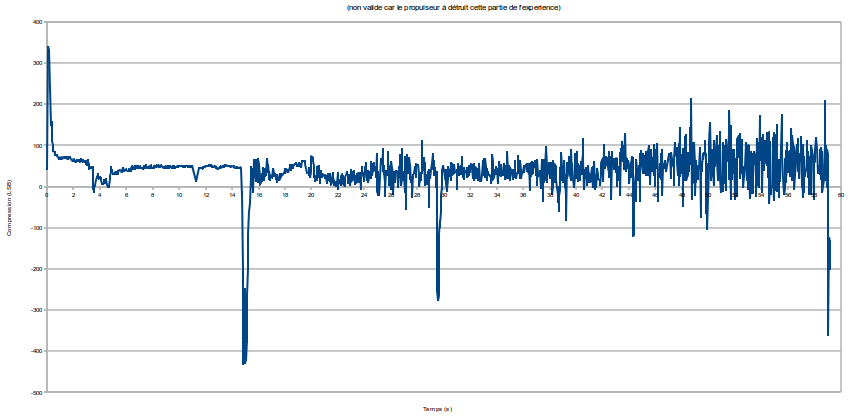
\includegraphics[height=208px, width=424px]{analyse/compression-ressort.png}
		\end{center}
	  \end{figure}		 
	  \subsubsection{Calcul du $C_x$}
	  Etant donné que nous n'avons pas de données valables pour l'expérience, nous ne pouvons pas calculer à partir de nos données expérimentales une valeur du $C_x$.
	  Nous pourrions toutefois obtenir une valeur en nous basant sur la poussée du constructeur théorique, et en dérivant deux fois l'altitude donnée par le capteur de pression pour avoir l'accélération.
	  Cependant la précision de ce calcul est indéterminable, donc cette valeur serait sans intérêt.
	 \newpage
	  \section{Conclusion}
	  
	  Ainsi s'achève cette aventure scientifique palpitante. On retiendra surtout du projet tout ce qu'il nous a appris.
	  D'un point de vue technique tout d'abord, avec la manipulation de machines outils (comme le tour par exemple) ou encore la conception d'un circuit électronique.
	  Construire une fusée c'est donc l'occasion de mettre en pratique des connaissances théoriques acquises au lycée.
	  C'est également une aventure humaine : Mercury résulte du travail d'une équipe qui s'est réunie chaque samedi de l'année dans les locaux de Eurêka+ à Marly-le-Roi et qui a vécu une semaine intense durant la campagne de lancement à Biscarrosse.
	  
	  On retiendra également l'erreur que nous avons commise sur le calcul du ressort. Après analyse, il semblerait que l'erreur vienne d'une mauvaise modélisation du problème, et nous vous invitons à lire l'annexe pour un calcul plus juste.

	  Modéliser correctement le comportement d'une fusée demande des outils de mécanique qui n'étaient pas à notre disposition en terminale.
	  
	  Enfin nous aimerions remercier l'équipe de Planète-Sciences pour le prix que nous avons reçu, ainsi que les animateurs de Eurêka+, Thibault et Adrien, sur lesquels toute l'association repose et sans lesquels l'aventure n'aurait pu décoller !

	  
	      \begin{figure}[H]
		    \begin{center}
		      \caption{Remise des prix le dernier jour.}
		      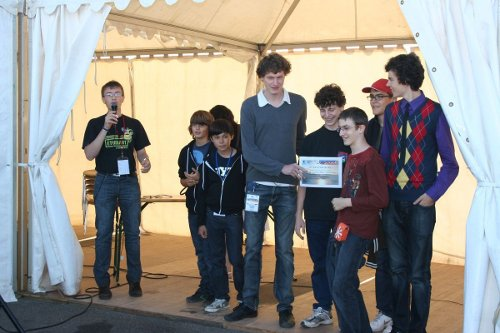
\includegraphics[height=217px, width=326px]{Photos_Mercury/remise_des_prix.jpg}
		    \end{center}
	      \end{figure}
	      \begin{figure}[H]
		    \begin{center}
		      \caption{Mercury remporte le prix Planète-Sciences !}
		      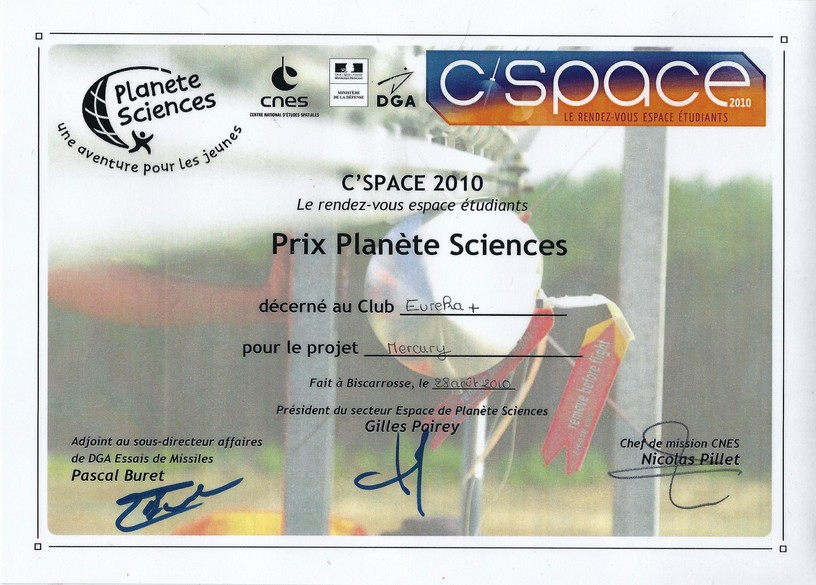
\includegraphics[height=244px, width=326px]{Photos_Mercury/Mercury_Prix_PS_2010.jpg}
		    \end{center}
	      \end{figure}
	\newpage
	\section{Annexe : dimensionnement du ressort}
	
    Dans le premier calcul du ressort que nous avons effectué (calcul présenté en partie 2.2) nous n'avons pas correctement défini le point sur lequel on appliquait le PFD, et nous avions fait des hypothèses fausses sur le comportement du ressort (qui pourtant nous semblaient logiques).
    Ce calcul est donc plus délicat que prévu, c'est pourquoi je l'ai refait ici, plusieurs mois après le vol, avec j'espère plus de précisions.
    
	\subsection{Etude théorique}
	L'objectif est de déterminer quel ressort choisir, c'est à dire quelle élongation $l_0$ et quelle raideur k choisir pour pouvoir 	mesurer le plus précisément possible la poussée du propulseur.


	En pratique $l_0$ doit être de l'ordre de 20 cm, j'essaye donc plutôt de calculer la constante k. \newpage

	\begin{wrapfigure}[23]{l}{7cm}
	\caption{Schéma du ressort dans le référentiel de la fusée à l'instant t}
	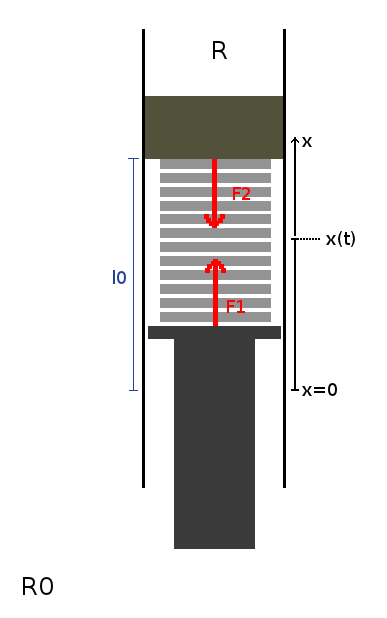
\includegraphics[width=5cm]{Photos_Mercury/schema_t.png}
	\end{wrapfigure}


	On distingue d'abord le référentiel lié à la Terre $R_0$ Galiléen et le référentiel lié à la fusée $R$ non Galiléen.

	On fait le bilan sur le ressort en appelant m sa masse, et x la position de son centre de gravité selon la longueur de la fusée, 	l'origine étant choisie pour correspondre au bas du ressort quand celui-ci ne subit aucune force (avant le décollage donc).

	On considère ensuite que le centre de gravité du ressort est au milieu de celui-ci.
	On a donc x(0) = l0 /2. 

	Le ressort subit  : 
	\begin{itemize}
	\item $\vec{F_1}$, la force du propulseur dont le constructeur donne une courbe expérimentale en fonction du temps (c'est un PRO-54).
	\item $\vec{F_2}$, la force exercée par la plaque de poussée (en verte kaki) sur le ressort
	\item La force d'inertie $-m \vec{a_e}$ où $\vec{a_e}$ est l'accélération subie par la fusée en son centre de gravité dans le 	référentiel R0, que l'on peut donc calculer en fonction du temps avec la méthode d'Euler pour les simulations en donnant une valeur 	"classique" au Cx comme 0.6 (et cette accélération sera mesurée en vrai).
	\item La force de Coriolis $-m\vec{\Omega} \wedge \vec{v_r}$, $\vec{\Omega}$ est la vecteur instantané de rotation donc $\vec{\Omega} = (\dot{\theta}, \dot{\varphi}, \dot{\psi})$ et $\vec{v_r}$ est la vitesse relation du ressort dans R donc $\vec{v_r} = (\dot{x}, 0, 0)$.
On a donc $\vec{\Omega} \wedge \vec{v_r} = (0, \dot{\psi} \dot{x}, \dot{\varphi} \dot{x})$.
En conclusion le produit vectoriel est nul sur l'axe des x : la force de Coriolis ne fait pas partie des forces subies par le ressort 

	\item Son poids projeté sur l'axe de la fusée : $-mg*\sin{\theta}$
	\end{itemize}

	En écrivant le PFD sur l'axe des x, on obtient donc : $$ m\ddot{x} = F_1 - F_2 -m{a_e}_x -mg*\sin{\theta}$$ où ${a_e}_x =$ projeté de $a_e$ sur l'axe de la fusée.

	En ce qui concerne F1 c'est la force du propulseur donc on peut l'estimer avec les données de poussées fournies par le constructeur 	du Pro-54.
	En ce qui concerne F2, on déduit son expression en appliquant la troisième loi de Newton sur la plaque de poussée : $-\vec{F2}$ est 	la force subie par la plaque de poussée du ressort. L'allongement du ressort est $2(l0-x(t))$ donc :
	$$F2 = k(l0-2x)$$


	Finalement en reportant on obtient : 

	$$F_{prop} + k(l0-2x) = m \ddot{x}+m{a_e}_x +mg\sin{\theta}$$ 

	avec $x(0) = l0/2$.

	Cette équation donne des conditions sur k.

	On souhaite de plus que quand le ressort est compressé au maximum, il y ait une différence de longueur avec la longueur à vide de 7cm : il s'agit de la différence d'élongation que l'on peut mesurer avec le potentiomètre (par exemple).

	J'ai donc $2 l_0 - 2(l_0-max(x)) = 7cm$ ie : $$max(x) = 3.5 cm$$
	Ceci est donc une contrainte supplémentaire sur k.

	\subsection{Simulation numérique}

	Pour trouver la valeur de k et calculer la position théorique du ressort à tout instant, on réalise une simulation numérique en 	Ocaml\footnote{Très bon langage de programmation enseigné en prépa}.

	On calcule les différentes valeurs en donnant une valeur classique au $C_x$ de 0.6.
	On calcule d'abord la position et l'accélération de la fusée sur sa longeur, ce qui correspont à ${a_e}$ puis la position du ressort 		à tout instant.

	Le code complet du programme peut être visionné ici : \url{https://github.com/robocop/Mercury}

	\subsection{Résultats}

	Pour la fusée qui a volé, on trouve k = 11880 N soit 5 fois plus que le ressort que nous avions choisit : 
	\begin{lstlisting}
$ ./calculs.native 
k = 11882.324219 N.m^-1
Sortie de rampe t : 0.31  h = 3.94 	 v = 27.24 theta = 79  a = 91.19 
Apogee          t : 15.73 h = 1328.00 v = 24.01 theta = 0	 a = -0.34 
	\end{lstlisting}

	A la place du ressort, on pourrait utiliser un capteur de distance infrarouge comme les Sharp gp2d120 pouvant mesurer une distance de 4 à 30 cm.
	\newpage
	
	On peut alors choisir un ressort de 30 cm et une différence d'élongation de 15 cm : 
	\begin{lstlisting}
$ ./calculs.native -l0 0.3 -l_potar 0.15
k = 6046.295166 N/m
Sortie de rampe t : 0.31  h = 3.94    v = 27.24 theta = 79  a = 91.19 
Apogee          t : 15.73 h = 1328.00 v = 24.01 theta = 0   a = -0.34 
	\end{lstlisting}
\end{document}
